\section{Attention model}
\label{sec:attention}

We now describe the our multi-focal attention model. We first introduce the optimization objective and inference, and then provide details on how scores are calculated and learned.

\subsection{Inference}
As noted earlier, the global score function in \eqref{eq:global_obj} is hard to maximize.
Here we simplify inference by decomposing the task over mentions. 
We choose this approach since integrating attention into it is simple in terms of both inference and learning.

%\begin{figure*}
%\begin{subfigure}[t]{.3\textwidth}
%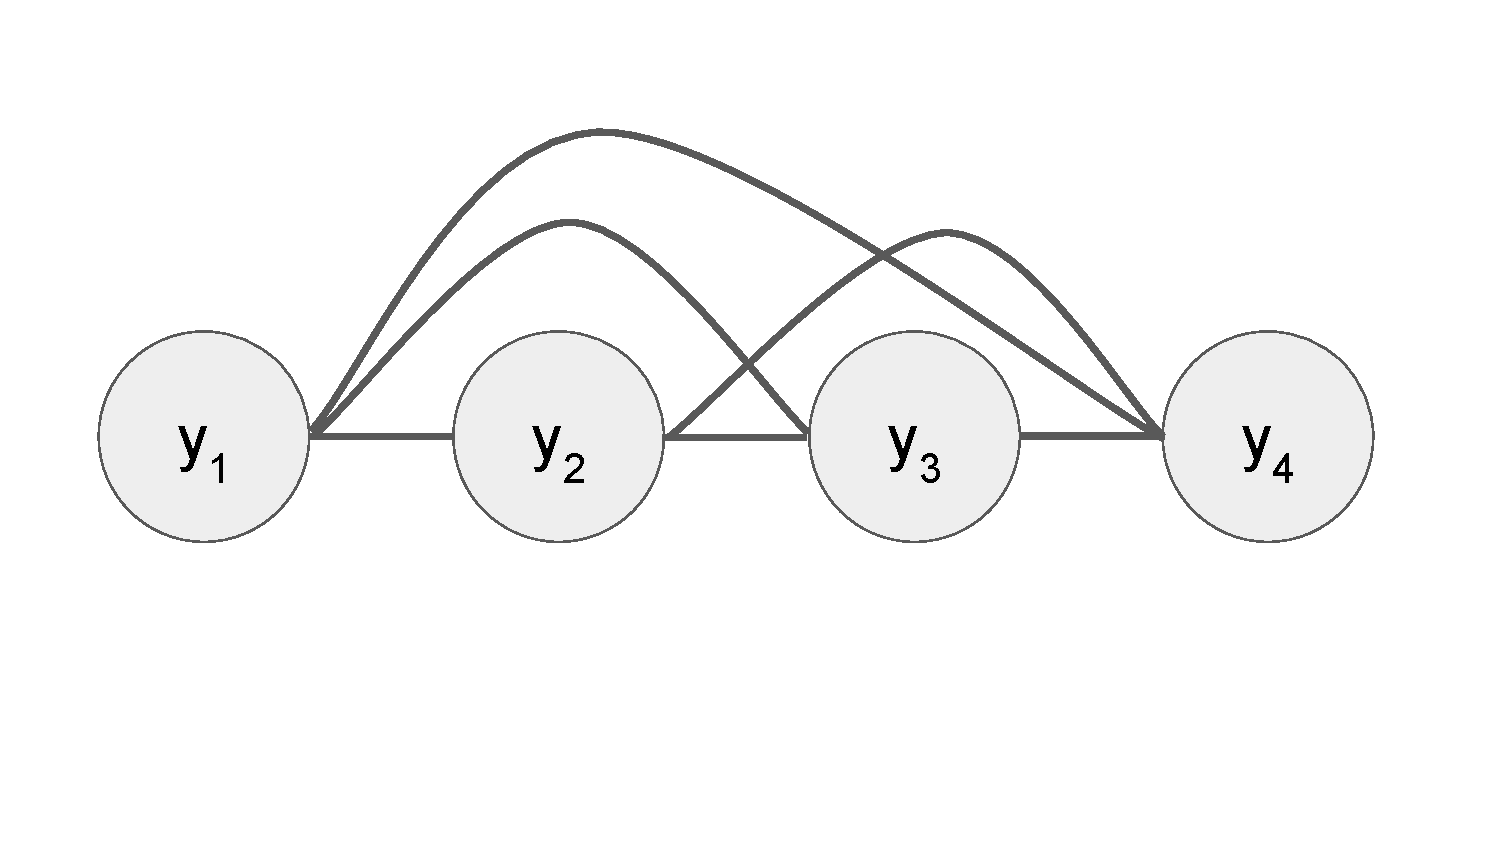
\includegraphics[width=\linewidth]{./complete_graph.pdf}
%\label{fig:fig_complete}
%\end{subfigure}
%\begin{subfigure}[t]{.3\textwidth}
%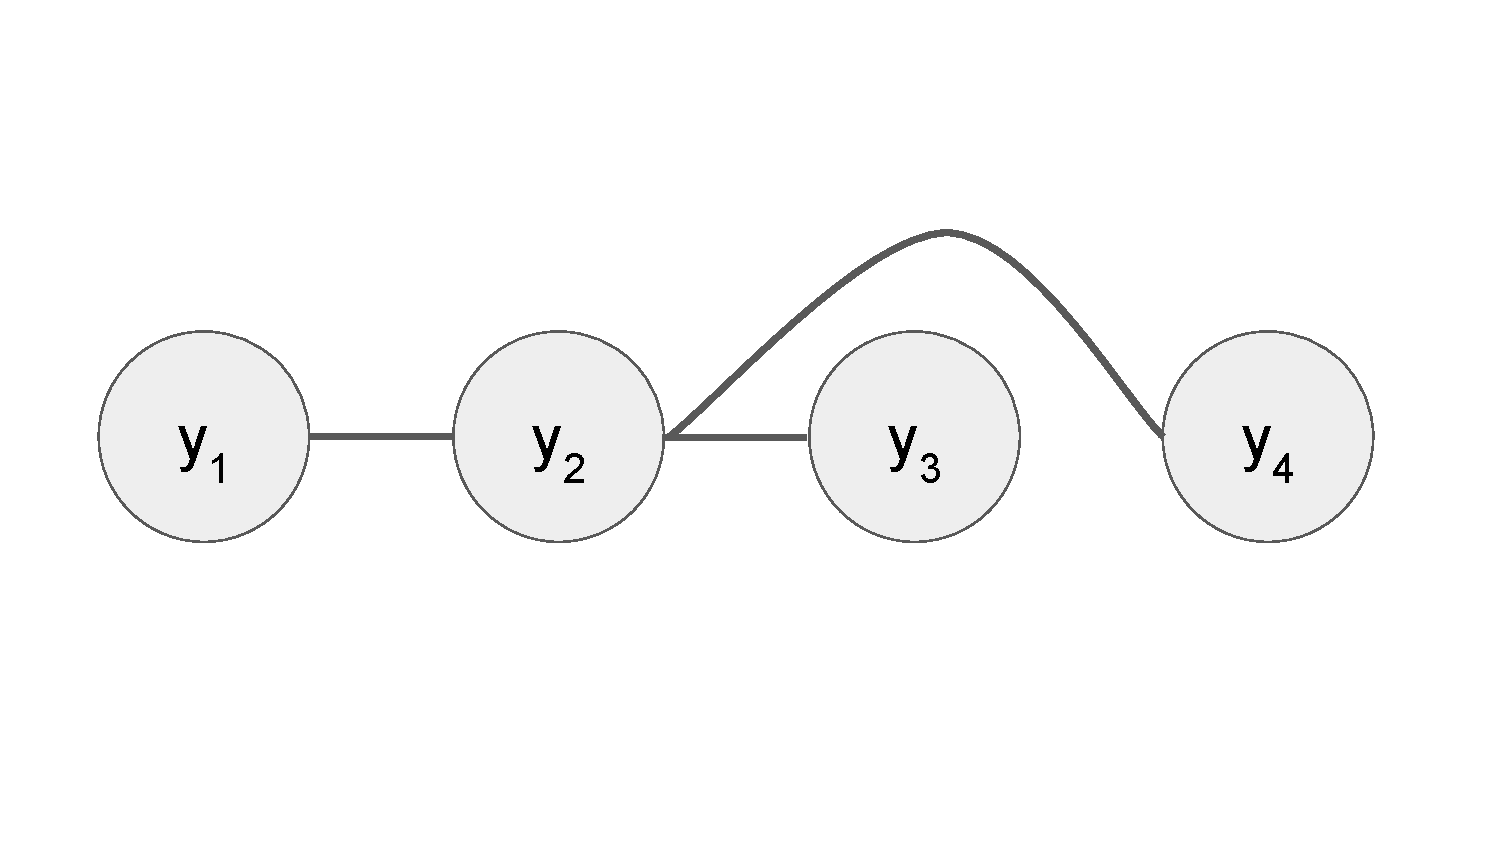
\includegraphics[width=\linewidth]{./y2_graph.pdf}
%\label{fig:fig_y2}
%\end{subfigure}
%\begin{subfigure}[t]{.3\textwidth}
%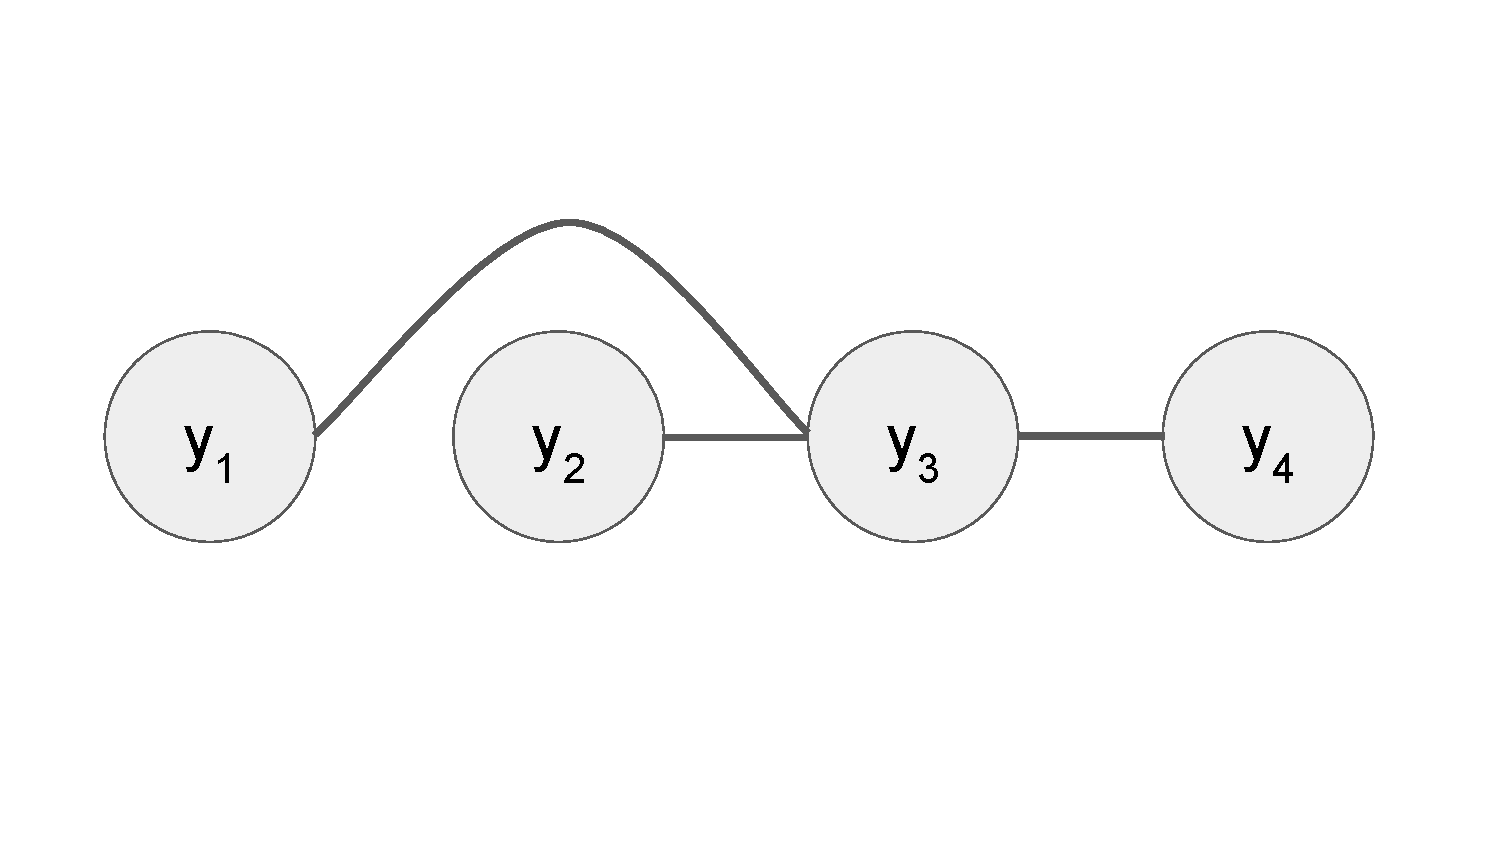
\includegraphics[width=\linewidth]{./y3_graph.pdf}
%\label{fig:fig_y3}
%\end{subfigure}
%%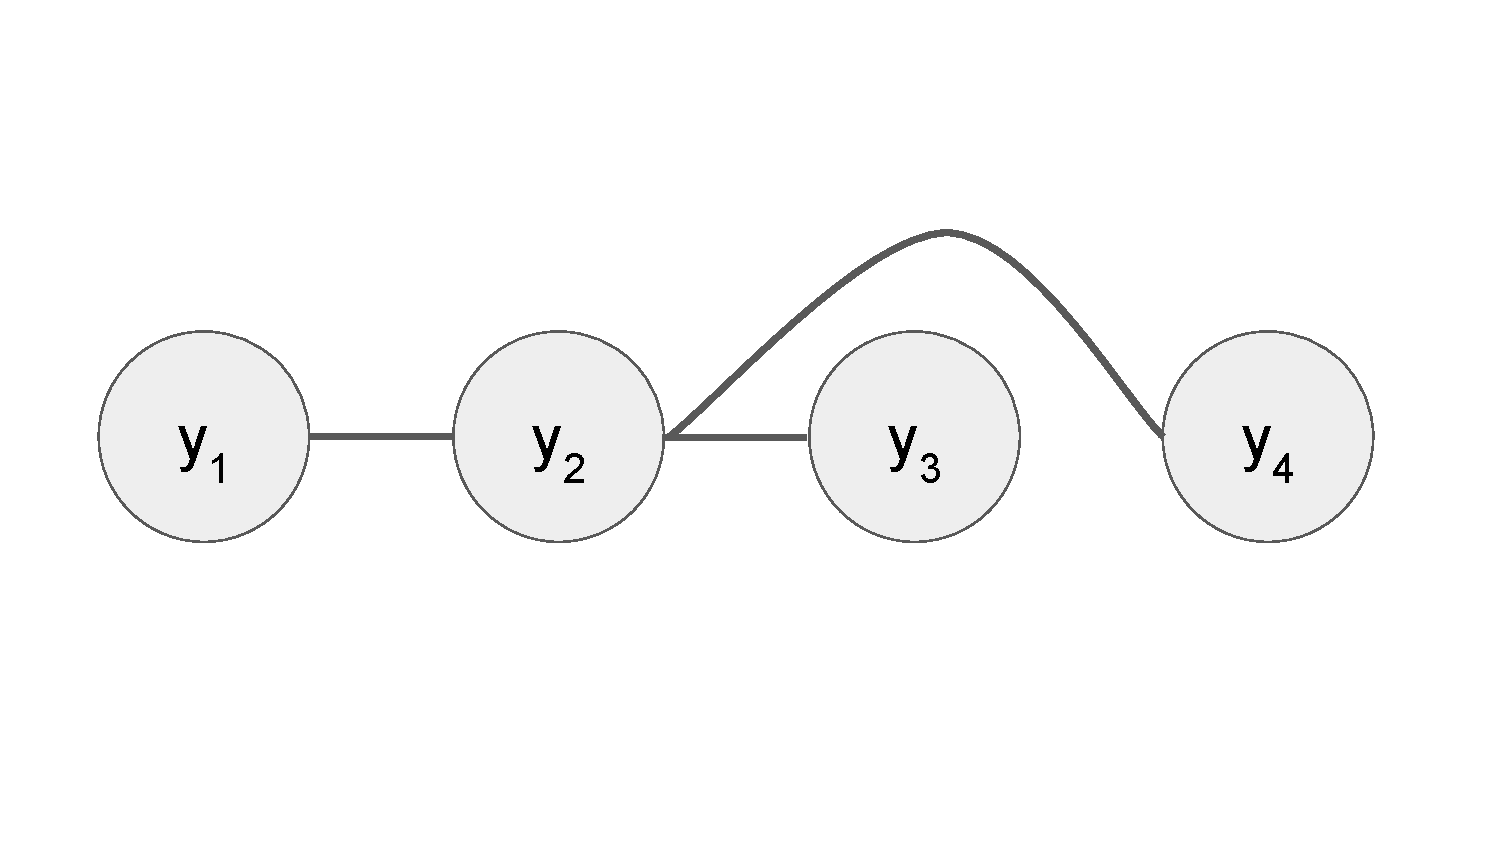
\includegraphics[width=2in]{./y2_graph.pdf}
%%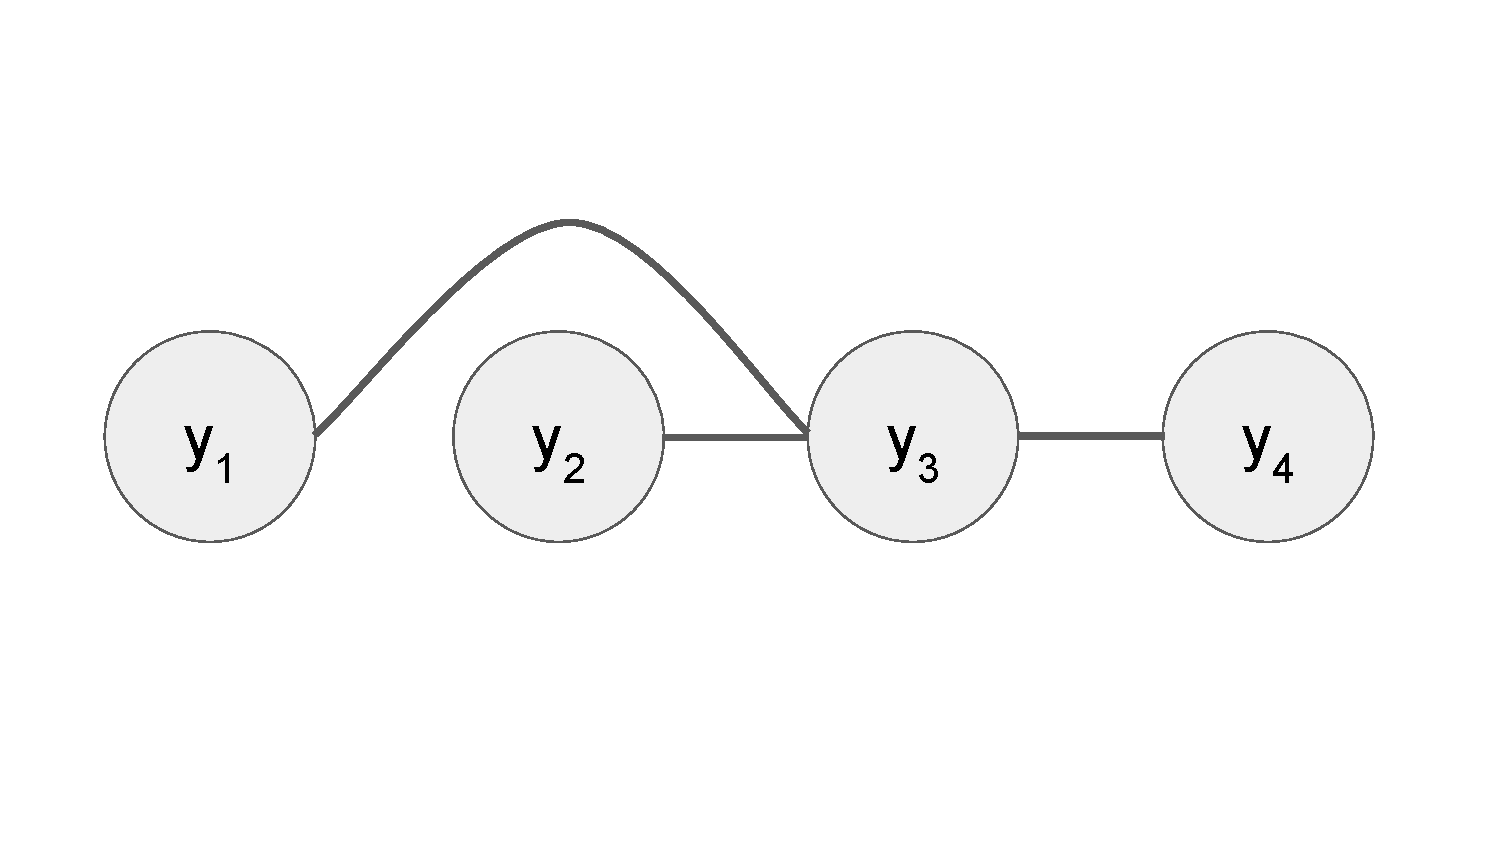
\includegraphics[width=2in]{./y3_graph.pdf}
%%\subfloat[The complete graph corresponding to \eqref{eq:global_obj}]
%%\subfloat[A star shaped subgraph corresponding to $y_2$. This will be used to obtaining the label $y_2$]
%\begin{minipage}[t]{\textwidth}
%\caption{{\bf Left:} The complete graph corresponding to \eqref{eq:global_obj}. {\bf Middle:}  A star shaped subgraph corresponding to $y_2$. This will be used to obtaining the label $y_2$. {\bf Right: } The star graph for $y_3$.}
%\label{fig:star}
%\end{minipage}
%\end{figure*}


\begin{figure}[t!]
\label{fig:model}
\begin{tikzpicture}[node distance=0.8cm and 1cm,>=stealth',auto]
\tikzstyle{candidate}=[circle,draw=black,fill=gray!10,font=\large]
  \tikzstyle{section}=[rectangle,minimum size=6mm,font=\large]
\begin{scope}[-,thick]

  \node[candidate]  (x1)      {$y_1$} ;
  \node[candidate, right=of x1] (x2) {$y_2$} ; 
  \node[candidate, right=of x2] (x3) {$y_3$} ; 
  \node[candidate, right=of x3] (x4) {$y_4$} ; 
  \node[section, left=0.1cm of x1] (a) {(a)};
  \path(x1.east) edge (x2.west);
  \path(x2.east) edge (x3.west);
  \path(x3.east) edge (x4.west);
  \path(x1.east) edge [bend left=45] (x3.west);
  \path(x2.east) edge [bend left=45] (x4.west);
    \path(x1.east) edge [bend left=45] (x4.west);

  \node[candidate, below=of x1]  (y1)      {$y_1$} ;
  \node[candidate, right=of y1] (y2) {$y_2$} ; 
  \node[candidate, right=of y2] (y3) {$y_3$} ; 
  \node[candidate, right=of y3] (y4) {$y_4$} ; 
    \node[section, left=0.1cm of y1] (b) {(b)};
  \path(y1.east) edge (y2.west);
  \path(y2.east) edge (y3.west);
  \path(y2.east) edge [bend left=45] (y4.west);
  
    \node[candidate, below=of y1]  (z1)      {$y_1$} ;
  \node[candidate, right=of z1] (z2) {$y_2$} ; 
  \node[candidate, right=of z2] (z3) {$y_3$} ; 
  \node[candidate, right=of z3] (z4) {$y_4$} ; 
    \node[section, left=0.1cm of z1] (c) {(c)};
  \path(z2.east) edge (z3.west);
  \path(z3.east) edge (z4.west);
  \path(z1.east) edge [bend left=45] (z3.west);
\end{scope}
\end{tikzpicture}
\caption{(a) The complete graph corresponding to \eqref{eq:global_obj}. (b) A star shaped subgraph corresponding to $y_2$. This will be used to obtaining the label $y_2$. (c) The star graph for $y_3$.}
\label{fig:star}
\end{figure}

\subsubsection{Star model}

We start by considering a simple attention-free model in which inference is tractable, which we call a {\em star model}. For a particular mention $i$ and entity $y_i$, the star model is a graphical model that contains $y_i$, all interactions between $y_i$ and other labels, and no other interactions, as illustrated in \figref{fig:star}. 
% In this approach, the entity $y_i$ for mention $i$ is obtained as follows. Consider a star-shaped graphical model centered at $y_i$, as illustrated in \figref{fig:star}. Namely, the graph that contains all interactions of $y_i$ with other labels, but not interactions between the other labels. 

While the star graph centered at $i$ contains up to $n$ variables, we will only use it to infer the label of mention $i$. 
%We propose to obtain label $y_i$
%by maximizing $f_i$ over all labels, and returning the label for $y_i$.
Let $q_{ij}(y_i)$ be the support for label $y_i$ from mention $j$, defined as follows:
\be
q_{ij}(y_i) = \max_{y_j}  s_{ij}(y_i,y_j)  + s_j(y_j),
\label{eq:q}
\ee
and we also define $q_{ii}(y_i)=-\infty$ to simplify notation for later. We define the following score function for mention $i$:
\be
f_i(y_i) = s_i(y_i) + \sum_{j:j\neq i} q_{ij}(y_i)
\label{eq:star_obj}
\ee
and predict the label $y_i = \arg \max_{y} f_i(y)$.


Due to the structure of the star graph, inference is easy and can be done in $O(nC^2)$, where $C$ is the maximum number of candidates. A similar decomposition has previously been used in the context of approximate learning for structured prediction~\cite{SontagNIPS10}. 

To summarize, we replace the hard problem of maximizing  \eqref{eq:global_obj} with $n$ simple problems of maximizing over star shaped graphs. Note that we do not view this approach as an approximation to the global problem, but rather as our inference procedure.

 

\subsubsection{Adding attention \label{sec:add_attention}}
The score function in \eqref{eq:star_obj} aggregates pairwise scores for each label $y_i$ over all mentions. In this section, we restrict this to only consider $K$ mentions with the strongest relations to $y_i$.\footnote{It is possible to relax this to allow {\em up to} $K$ relations, but we focus on exactly $K$ for simplicity.} 
  Let $\amax_K({\bf z})$  be the sum of the largest $K$ values in the vector
${\bf z} = (z_1,\ldots,z_n)$.  For each label $y_i$,
we redefine the score function to be
% Thus, $q_{ij}(y_i)$ gives the strength of support that mention $j$
% gives to candidate $y_i$, for the best choice of $y_j$.  Since we want
% to only attend to the most informative mentions, we will only consider
% the $K$ best mentions. Namely, we consider the score function:
\be
f_i(y_i) = s_i(y_i) + \amax_K({\bf q}_i (y_i)),
\label{eq:amax_obj}
\ee
where ${\bf q}_i(y_i) = (q_{i1}(y_i), \ldots, q_{in}(y_i))$ and $q_{ij}(y_i)$ is as defined in \eqref{eq:q}.
The inference rule is again $y_i = \arg\max_y f_i(y)$, and the computational cost is $O(nC^2+ n\log{n})$ since sorting is required.\footnote{Note that if $K < \log{n}$, we spend only $nK$ instead of $n\log{n}$ time.}


\subsubsection{Soft attention}
\label{sec:soft_attention}

Several works on attention have shown that it is better to use a soft form of attention, where the level of attention is not zero or one, but can rather take intermediate values. In current attention models, the attention is to a single object, such as a single word \cite{bahdanau2014neural} or a single image window \cite{xu2015show}. In these cases, it is natural to change the max function in the attention operator to a soft-max. In our case, the attention beam contains $K$ elements, and we require a different notion of a soft-max, which we develop below.

Our goal is to obtain a soft version of the function  $\amax_K({\bf z})$. To do so, we first use an alternative definition of this function, as the solution 
to the optimization problem:
\be
 \max_{ 
\begin{array}{l}
x_1,\ldots,x_n: \\
0 \leq x_i \leq 1\\
 \sum_i x_i = K
 \end{array}
 } \sum_i z_i x_i
\ee
The optimization problem above is a linear program, whose solution is the sum of top $K$ elements of ${\bf z}$ as required. This follows since optimal $x_i$ can easily be shown to attain only integral values (otherwise the objective can be improved). Alternatively, it can be shown that the vertices of the constraining polytope are integral.

Given this optimization view of $\amax_K({\bf z})$ it is natural to smooth it \cite{nesterov2005smooth} by adding a non-linearity to the optimization. Since the variables are non-negative, one possible choice is an entropy-like regularizer\footnote{Note that $-\sum_i x_i \log x_i$ is different from the entropy function since variables $x_i$ sum to $K$ and not to 1.}. We shall see that this choice results in a closed form solution, and also recovers the standard soft-max case for $K=1$.  Consider the optimization problem:
\be
 \max_{ 
\begin{array}{l}
x_1,\ldots,x_n: \\
0 \leq x_i \leq 1\\
 \sum_i x_i = K
 \end{array}
 } \sum_i z_i x_i - \beta^{-1} \sum_i x_i \log{x_i},
 \label{eq:softkmax_opt}
 \ee
 where $\beta$ is a tuned hyperparameter.  We denote the solution by $\samax_K({\bf z})$. The following proposition provides a closed form solution for $\samax_K$, as well as its gradient.

\begin{proposition}
 \label{prop:softkmax}
Assume $i_1,\ldots,i_n$ are such that $z_{i_1}\geq \ldots \geq z_{i_n}$. Then:
\be
\samax_K({\bf z}) = \sum_{j=1}^{K-1} z_{i_j} + \beta^{-1} \log\sum_{j=K}^n \expo{\beta z_{i_j}}  
\ee
The function $\samax_K({\bf z})$ is differentiable. Denote its gradient with respect to $z_i$ by $v_i$. Also, define:
\bea
c &=& \beta^{-1} \log\sum_{j=K}^n \expo{\beta z_{i_j}} \\
d &=& (K-1) \expo{\beta c} + \sum_{j=K}^n \expo{\beta z_{i_j}}
\eea
Then $v_i$ is given by:
\be
v_{i_j} =
\left\{
\begin{array}{ll}
\frac{\expo{\beta c}}{d} & j = 1,\ldots,K-1 \\
\frac{\expo{\beta z_{i_j}}}{d} & j = K,\ldots,n 
\end{array} 
\right\}
\ee
\end{proposition}  
\noindent Proof is provided in the appendix.

As noted, $K=1$ recovers the standard soft-max function.\footnote{When we refer to the {\em soft-max function}, we mean the function $\beta^{-1}\log\sum \expo{\beta a_i}$, which is an often used differentiable convex upper bound of the max function (e.g., see \cite{gimpel2010softmax}). Soft-max sometimes
also refers to the activation function $\frac{\expo{a_i}}{\sum_{j} \expo{a_j}}$. The latter is in fact the gradient of the former (for $\beta=1$). } For other values of $K$, the function $\samax_K$ has an intuitive interpretation: take the sum of the top $K-1$ elements of $z_1,\ldots,z_n$, and add the soft-max of all other elements. As $\beta \to \infty$, this soft-max will approach the true max and therefore the soft-max of the suffix will be exactly the $K^{th}$ top element, and $\samax_K$ will therefore be the sum of the top $K$ elements as expected. For  finite $\beta$ we have a soft version of $\amax_K$.

Our soft attention based model will therefore consider the soft-variant of \eqref{eq:amax_obj}:
\be
f_i(y_i) = s_i(y_i) + \samax_K({\bf q}_{i}(y_i)) ~,
\label{eq:samax_obj}
\ee
and maximize $f(y_i)$ to obtain the label.
 
\subsection{Score parameterization \label{sec:score_param}}
Thus far we assumed the singelton and pairwise scores were given. As in other structured prediction works, we will assume that the scores are features of the input and labels. Specifically, denote a set of singleton features by $\fs\in\reals^{n_s}$ and a set of pairwise features by $\fp\in\reals^{n_p}$. Then the model has two sets of weights $\ws$ and $\wp$ and the scores are obtained as a linear combination of the features. Namely:
\bea
s_i(y_i;\ws) &=& \ws\cdot\fs  \\
s_{ij}(y_i,y_j;\wp) &=& \wp\cdot\fp ~,
\eea
where we have explicitly denoted the dependence of the scores on the weight vectors.  See \secref{sec:expt:features} for details on how the features are chosen. It is of course possible to consider non-linear alternatives for the score function, as in recent deep learning parsing models \cite{chen2014fast,neurosis}, but we focus on the linear case for simplicity.

\subsection{Parameter learning \label{sec:learning}}
The parameters $\ws,\wp$ are learned from labeled data, as explained next. Since prediction is performed for each mention separately, we use a simple hinge loss for that mention. The loss is defined as follows. Denote by $y^*_i$ the ground
truth label for mention $i$. Define the corresponding ground truth pairwise score as:
\be
s^*_{ij} = s_{ij}(y^*_i,y^*_j)
\ee
Then the hinge loss is:
\bea
\ell_i &=& \max_{y_i}[ s_i(y_i) + \samax_K(s_{i1}(y_i), \ldots, s_{in}(y_i))  \\
       && - s_i(y^*_i) - \samax_K(s^*_{i1}, \ldots, s^*_{in})  
       + \Delta(y_i,y^*_i) ]
\eea
where $\Delta(y_i,y^*_i)$ is zero if $y_i=y^*_i$ and one otherwise.

The overall loss is simply the sum of losses for all the mentions, plus $\ell_2$ regularization over $\ws,\wp$. To minimize the loss we use AdaGrad \cite{adagrad} with learning rate $\eta=0.1$.


%%% Local Variables: ***
%%% mode:latex ***
%%% TeX-master: "main.tex"  ***
%%% tex-main-file: "main.tex"  ***
%%% End: ***
